\usepackage{tikz}

\counterwithout{figure}{section}
\counterwithout{table}{section}
\counterwithout{equation}{section}

\titleformat{\subsection}[block]
  {\bfseries\filcenter}{#1}{0cm}{}
\titlespacing{\subsection}{0cm}{21pt}{21pt}

\DeclareCaptionLabelFormat{gosttable}{Таблица #2}

\usepackage{float}
\usepackage{pgfplots}
\usepackage{graphicx}
\usepackage{multirow}
\usepackage{amssymb,amsfonts,amsmath,amsthm}

\usepackage{listings}
\lstset{basicstyle=\footnotesize\ttfamily,breaklines=true}
\lstset{language=Matlab}


\newcommand{\labnumber}{6} % sixth lab
\usepackage{tikz}

\counterwithout{figure}{section}
\counterwithout{table}{section}
\counterwithout{equation}{section}

\titleformat{\subsection}[block]
  {\bfseries\filcenter}{#1}{0cm}{}
\titlespacing{\subsection}{0cm}{21pt}{21pt}

\DeclareCaptionLabelFormat{gosttable}{Таблица #2}

\newcommand{\khpistudentgroup}{2.КН201н.8а}
\newcommand{\khpistudentname}{Чепурний~А.~С.}

\newcommand{\khpidepartment}{Програмна інженерія та інформаційні технології управління}
\newcommand{\khpititlewhat}{
	Розрахунково-графічне завдання \\
	з предмету <<Фреймворки та платформи>>
}
\newcommand{\khpititlewho}{
	Виконав: \\
	\hspace*{\parindent} ст. групи \khpistudentgroup \\
	\hspace*{\parindent} \khpistudentname \\
	Перевірила: \\
	\hspace*{\parindent} к. т. н., вик. каф. ПІІТУ \\
	\hspace*{\parindent} Добряк~В.~С. \\
}


\usepackage{systeme}
\usepackage{longtable,tabu}
\usepackage{multirow}
\usepackage{array,multirow}
\usepackage{pdflscape}
\usepackage{afterpage}
\usepackage{tikz}
\usepackage{bm}
\usepackage{qtree}

\graphicspath{{figures/}}

\begin{document}
\Russian

\begin{titlepage}

\begin{center}
	МІНІСТЕРСТВО ОСВІТИ І НАУКИ УКРАЇНИ \\
	НАЦІОНАЛЬНИЙ ТЕХНІЧНИЙ УНІВЕРСИТЕТ \\
	«ХАРКІВСЬКИЙ ПОЛІТЕХНІЧНИЙ ІНСТИТУТ» \\
	Кафедра <<\khpidepartment>> \\
\end{center}

\vspace{6cm}

\begin{center}
	\khpititlewhat
\end{center}

\vspace{3cm}

\begin{addmargin}[10cm]{0cm}
	\khpititlewho
\end{addmargin}

\vspace{\fill}

\begin{center}
	Харків \the\year
\end{center}

\end{titlepage}

\addtocounter{page}{1}

\textbf{Тема}: оценка и упорядочение альтернатив при аддитивности критериев.

\textbf{Цель}: 
\begin{itemize}
	\item изучить теоретические основы по оценке и упорядочении альтернатив при аддитивности критериев;
	\item закрепить теоретические знания решением практической задачи;
	\item провести анализ полученных результатов и сделать выводы по работе.
\end{itemize}

\textbf{Задание}: 
Самостоятельно сформировать задачу исследования. Включить 4 критерия и 4 альтернативы. Решить задачу исследования в соответствии с предложенной методикой. При выполнение арифметических операций над нечеткими числами использовать методику, рассмотренную ранее (построить все функции).

Провести анализ полученных результатов.

\textbf{Исходные данные}: 
Оценки четырех альтернатив приведены в таблице~\ref{tab:source}.

\begin{table}[H]
	\caption{Критериальные оценки для четырех альтернатив}
	\label{tab:source}
	\begin{tabular}{l|llll}
		           & Голубой & Сиреневый & Салатный & Красный \\\hline
		Красный    & Плохо & Средне & Плохо & Хорошо \\
		Зеленый    & Средне & Плохо & Хорошо & Плохо \\
		Синий      & Хорошо & Хорошо & Средне & Плохо \\
		Прозрачный & Плохо & Плохо & Плохо & Плохо \\
	\end{tabular}
\end{table}

Первый критерий определен как \textit{СРЕДНЕЙ ВАЖНОСТИ} ($W_2$), второй --- \textit{НЕ ОЧЕНЬ ВАЖНЫЙ} ($W_1$), третий --- \textit{ОЧЕНЬ ВАЖНЫЙ} ($W_4$), четвертый --- \textit{ДОВОЛЬНО ВАЖНЫЙ} ($W_3$). 
Термы заданы функциями принадлежности, представленными на рисунке~\ref{fig:source_1} и~\ref{fig:source_2}.

\begin{figure}[H]
	\centering
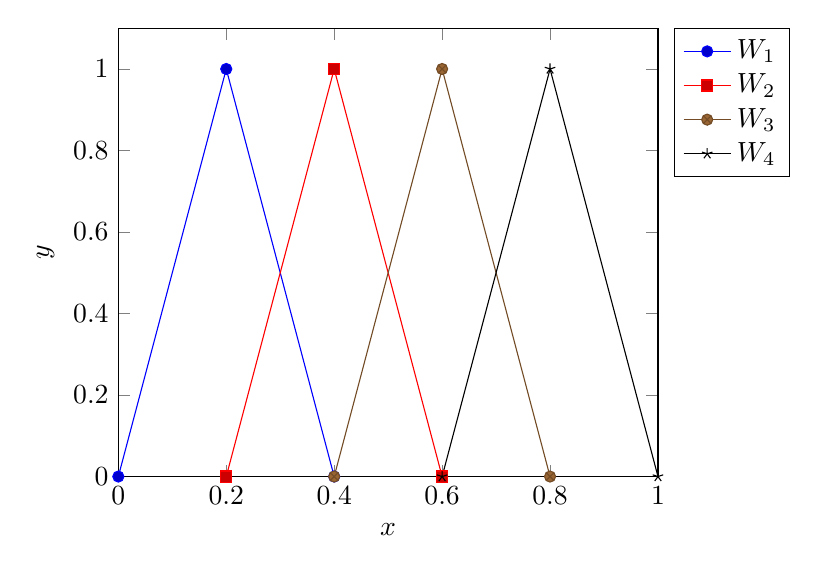
\begin{tikzpicture}
	\begin{axis}[
		legend pos=outer north east,
		ymin=0,
		xmin=0,
		xmax=1,
		xlabel=$x$,
		ylabel=$y$,]
		\addplot coordinates {(0.0,0.0) (0.2,1.0) (0.4,0.0)};
		\addlegendentry{$W_1$}
		\addplot coordinates {(0.2,0.0) (0.4,1.0) (0.6,0.0)};
		\addlegendentry{$W_2$}
		\addplot coordinates {(0.4,0.0) (0.6,1.0) (0.8,0.0)};
		\addlegendentry{$W_3$}
		\addplot coordinates {(0.6,0.0) (0.8,1.0) (1.0,0.0)};
		\addlegendentry{$W_4$}
	\end{axis}
\end{tikzpicture}
	\caption{Функции принадлежности коэффициентов важности $W_1$, $W_2$, $W_3$, $W_4$}
	\label{fig:source_1}
\end{figure}

\begin{figure}[H]
	\centering
\begin{tikzpicture}
	\begin{axis}[
		legend pos=outer north east,
		ymin=0,
		xmin=0,
		xmax=1,
		xlabel=$x$,
		ylabel=$y$,]
		\addplot coordinates {(0.0,0.0) (0.2,1.0) (0.4,0.0)};
		\addlegendentry{Плохо}
		\addplot coordinates {(0.3,0.0) (0.5,1.0) (0.7,0.0)};
		\addlegendentry{Средне}
		\addplot coordinates {(0.6,0.0) (0.8,1.0) (1.0,0.0)};
		\addlegendentry{Хорошо}
	\end{axis}
\end{tikzpicture}
	\caption{Функции принадлежности критериальных оценок для случая четырех альтернатив}
	\label{fig:source_2}
\end{figure}

\subsection{Ход работы}

Расчитаем умножения коэфициентов важности и критериальных оценок:
\begin{multline*}
	\textup{Красный}_\textup{Плохо} = W_2 \times \textup{Плохо} = \\ = \{ <0.0, 0.2>, <1.0, 0.4>, <0.0, 0.6> \} \times \\ \times \{ <0.0, 0.0>, <1.0, 0.2>, <0.0, 0.4> \} = \\ = \{ <0.0, 0.04>, <1.0, 0.08>,	<0.0, 0.12> \},
\end{multline*}
\begin{multline*}
	\textup{Красный}_\textup{Средне} = W_2 \times \textup{Средне} = \\ = \{ <0.0, 0.2>, <1.0, 0.4>, <0.0, 0.6> \} \times \\ \times \{ <0.0, 0.3>, <1.0, 0.5>, <0.0, 0.8> \} = \\ = \{ <0.0, 0.18>, <1.0, 0.2>,	<0.0, 0.28> \},
\end{multline*}
\begin{multline*}
	\textup{Красный}_\textup{Хорошо} = W_2 \times \textup{Хорошо} = \\ = \{ <0.0, 0.2>, <1.0, 0.4>, <0.0, 0.6> \} \times \\ \times \{ <0.0, 0.6>, <1.0, 0.8>, <0.0, 1.0> \} = \\ = \{ <0.0, 0.24>, <1.0, 0.32>,	<0.0, 0.36> \},
\end{multline*}
\begin{multline*}
	\textup{Зеленый}_\textup{Плохо} = W_1 \times \textup{Плохо} = \\ = \{ <0.0, 0.0>, <1.0, 0.2>, <0.0, 0.4> \} \times \\ \times \{ <0.0, 0.0>, <1.0, 0.2>, <0.0, 0.4> \} = \\ = \{ <0.0, 0.0>, <1.0, 0.04>,	<0.0, 0.08> \},
\end{multline*}
\begin{multline*}
	\textup{Зеленый}_\textup{Средне} = W_1 \times \textup{Средне} = \\ = \{ <0.0, 0.0>, <1.0, 0.2>, <0.0, 0.4> \} \times \\ \times \{ <0.0, 0.3>, <1.0, 0.5>, <0.0, 0.8> \} = \\ = \{ <0.0, 0.06>, <1.0, 0.1>,	<0.0, 0.12> \},
\end{multline*}
\begin{multline*}
	\textup{Зеленый}_\textup{Хорошо} = W_1 \times \textup{Хорошо} = \\ = \{ <0.0, 0.0>, <1.0, 0.2>, <0.0, 0.4> \} \times \\ \times \{ <0.0, 0.6>, <1.0, 0.8>, <0.0, 1.0> \} = \\ = \{ <0.0, 0.12>, <1.0, 0.16>,	<0.0, 0.2> \},
\end{multline*}
\begin{multline*}
	\textup{Синий}_\textup{Плохо} = W_4 \times \textup{Плохо} = \\ = \{ <0.0, 0.6>, <1.0, 0.8>, <0.0, 1.0> \} \times \\ \times \{ <0.0, 0.0>, <1.0, 0.2>, <0.0, 0.4> \} = \\ = \{ <0.0, 0.12>, <1.0, 0.16>,	<0.0, 0.2> \},
\end{multline*}
\begin{multline*}
	\textup{Синий}_\textup{Средне} = W_4 \times \textup{Средне} = \\ = \{ <0.0, 0.6>, <1.0, 0.8>, <0.0, 1.0> \} \times \\ \times \{ <0.0, 0.3>, <1.0, 0.5>, <0.0, 0.8> \} = \\ = \{ <0.0, 0.3>, <1.0, 0.4>,	<0.0, 0.42> \},
\end{multline*}
\begin{multline*}
	\textup{Синий}_\textup{Хорошо} = W_4 \times \textup{Хорошо} = \\ = \{ <0.0, 0.6>, <1.0, 0.8>, <0.0, 1.0> \} \times \\ \times \{ <0.0, 0.6>, <1.0, 0.8>, <0.0, 1.0> \} = \\ = \{ <0.0, 0.6>, <1.0, 0.64>,	<0.0, 0.8> \},
\end{multline*}
\begin{multline*}
	\textup{Прозрачный}_\textup{Плохо} = W_3 \times \textup{Плохо} = \\ = \{ <0.0, 0.4>, <1.0, 0.6>, <0.0, 0.8> \} \times \\ \times \{ <0.0, 0.0>, <1.0, 0.2>, <0.0, 0.4> \} = \\ = \{ <0.0, 0.08>, <1.0, 0.12>,	<0.0, 0.16> \},
\end{multline*}
\begin{multline*}
	\textup{Прозрачный}_\textup{Средне} = W_3 \times \textup{Средне} = \\ = \{ <0.0, 0.4>, <1.0, 0.6>, <0.0, 0.8> \} \times \\ \times \{ <0.0, 0.3>, <1.0, 0.5>, <0.0, 0.8> \} = \\ = \{ <0.0, 0.28>, <1.0, 0.3>,	<0.0, 0.4> \},
\end{multline*}
\begin{multline*}
	\textup{Прозрачный}_\textup{Хорошо} = W_3 \times \textup{Хорошо} = \\ = \{ <0.0, 0.4>, <1.0, 0.6>, <0.0, 0.8> \} \times \\ \times \{ <0.0, 0.6>, <1.0, 0.8>, <0.0, 1.0> \} = \\ = \{ <0.0, 0.4>, <1.0, 0.48>,	<0.0, 0.6> \}.
\end{multline*}

Тогда взвешенные оценки равны (рисунок~\ref{fig:result}):
\begin{multline*}
	\textup{Голубой} = \textup{Красный}_\textup{Плохо} + \textup{Зеленый}_\textup{Средне} + \\ + \textup{Синий}_\textup{Хорошо} + \textup{Прозрачный}_\textup{Плохо} = \\ = \{ <0.0, 0.36>, <1.0, 0.94>,	<0.0, 1.84> \},
\end{multline*}
\begin{multline*}
	\textup{Сиреневый} = \textup{Красный}_\textup{Средне} + \textup{Зеленый}_\textup{Плохо} + \\ + \textup{Синий}_\textup{Хорошо} + \textup{Прозрачный}_\textup{Плохо} = \\ = \{ <0.0, 0.42>, <1.0, 1.0>,	<0.0, 1.9> \},
\end{multline*}
\begin{multline*}
	\textup{Салатный} = \textup{Красный}_\textup{Плохо} + \textup{Зеленый}_\textup{Хорошо} + \\ + \textup{Синий}_\textup{Средне} + \textup{Прозрачный}_\textup{Плохо} = \\ = \{ <0.0, 0.18>, <1.0, 0.76>,	<0.0, 1.66> \},
\end{multline*}
\begin{multline*}
	\textup{Красный} = \textup{Красный}_\textup{Хорошо} + \textup{Зеленый}_\textup{Плохо} + \\ + \textup{Синий}_\textup{Плохо} + \textup{Прозрачный}_\textup{Плохо} = \\ = \{ <0.0, 0.12>, <1.0, 0.64>,	<0.0, 1.48> \}.
\end{multline*}

\begin{figure}[H]
	\centering
\begin{tikzpicture}
	\begin{axis}[
		legend pos=outer north east,
		ymin=0,
		xmin=0,
		xlabel=$x$,
		ylabel=$y$,]
		\addplot coordinates {(0.36,0.0) (0.94,1.0) (1.84,0.0)};
		\addlegendentry{Голубой}
		\addplot coordinates {(0.42,0.0) (1.0,1.0) (1.9,0.0)};
		\addlegendentry{Сиреневый}
		\addplot coordinates {(0.18,0.0) (0.76,1.0) (1.66,0.0)};
		\addlegendentry{Салатный}
		\addplot coordinates {(0.12,0.0) (0.64,1.0) (1.48,0.0)};
		\addlegendentry{Красный}
	\end{axis}
\end{tikzpicture}
	\caption{Взвешенные оценки альтернатив}
	\label{fig:result}
\end{figure}

Следовательно, наилучшей является вторая альтернатива, а потом первая, третья и четвертая.

\subsection{Выводы}

При выполнении лабораторной работы были изучены теоретические основы по оценке и упорядочении альтернатив при аддитивности критериев, затем теоретические знания были закреплены решением практической задачи.

\end{document}
